
% This is "sig-alternate.tex" V2.1 April 2013
% This file should be compiled with V2.5 of "sig-alternate.cls" May 2012
%
% This example file demonstrates the use of the 'sig-alternate.cls'
% V2.5 LaTeX2e document class file. It is for those submitting
% articles to ACM Conference Proceedings WHO DO NOT WISH TO
% STRICTLY ADHERE TO THE SIGS (PUBS-BOARD-ENDORSED) STYLE.
% The 'sig-alternate.cls' file will produce a similar-looking,
% albeit, 'tighter' paper resulting in, invariably, fewer pages.
%
% ----------------------------------------------------------------------------------------------------------------
% This .tex file (and associated .cls V2.5) produces:
%       1) The Permission Statement
%       2) The Conference (location) Info information
%       3) The Copyright Line with ACM data
%       4) NO page numbers
%
% as against the acm_proc_article-sp.cls file which
% DOES NOT produce 1) thru' 3) above.
%
% Using 'sig-alternate.cls' you have control, however, from within
% the source .tex file, over both the CopyrightYear
% (defaulted to 200X) and the ACM Copyright Data
% (defaulted to X-XXXXX-XX-X/XX/XX).
% e.g.
% \CopyrightYear{2007} will cause 2007 to appear in the copyright line.
% \crdata{0-12345-67-8/90/12} will cause 0-12345-67-8/90/12 to appear in the copyright line.
%
% ---------------------------------------------------------------------------------------------------------------
% This .tex source is an example which *does* use
% the .bib file (from which the .bbl file % is produced).
% REMEMBER HOWEVER: After having produced the .bbl file,
% and prior to final submission, you *NEED* to 'insert'
% your .bbl file into your source .tex file so as to provide
% ONE 'self-contained' source file.
%
% ================= IF YOU HAVE QUESTIONS =======================
% Questions regarding the SIGS styles, SIGS policies and
% procedures, Conferences etc. should be sent to
% Adrienne Griscti (griscti@acm.org)
%
% Technical questions _only_ to
% Gerald Murray (murray@hq.acm.org)
% ===============================================================
%
% For tracking purposes - this is V2.0 - May 2012

\documentclass{sig-alternate-05-2015}

\input{../preamble/preamble_nice.tex}
\DeclareRobustCommand{\mb}[1]{\ensuremath{\boldsymbol{\mathbf{#1}}}}

\DeclareMathOperator*{\argmax}{arg\,max}
\DeclareMathOperator*{\argmin}{arg\,min}

\DeclareRobustCommand{\KL}[2]{\ensuremath{\textrm{KL}\left(#1\;\|\;#2\right)}}

\newcommand{\mbx}{\mathbold{x}}
\newcommand{\mbX}{\mbf{X}}

\newcommand{\mbz}{\mathbold{z}}

\newcommand{\mbI}{\mbf{I}}

\newcommand{\mbZ}{\mbf{Z}}
\newcommand{\mbL}{\mbf{L}}

\newcommand{\mbtheta}{\mathbold{\theta}}
\newcommand{\mbTheta}{\mathbold{\Theta}}
\newcommand{\mbomega}{\mathbold{\omega}}
\newcommand{\mbOmega}{\mathbold{\Omega}}
\newcommand{\mbsigma}{\mathbold{\sigma}}
\newcommand{\mbSigma}{\mathbold{\Sigma}}

\newcommand{\mblambda}{\mathbold{\lambda}}
\newcommand{\mbgamma}{\mathbold{\gamma}}
\newcommand{\mbzeta}{\mathbold{\zeta}}
\newcommand{\mbeta}{\mathbold{\eta}}
\newcommand{\mbbeta}{\mathbold{\beta}}
\newcommand{\mbphi}{\mathbold{\phi}}
\newcommand{\mbmu}{\mathbold{\mu}}
\newcommand{\mbrho}{\mathbold{\rho}}

\newcommand\dif{\mathop{}\!\mathrm{d}}
\newcommand{\diag}{\textrm{diag}}
\newcommand{\supp}{\textrm{supp}}

\newcommand{\E}{\mathbb{E}}
\newcommand{\Var}{\mathbb{V}\textrm{ar}}

\newcommand{\bbN}{\mathbb{N}}
\newcommand{\bbZ}{\mathbb{Z}}
\newcommand{\bbR}{\mathbb{R}}
\newcommand{\bbS}{\mathbb{S}}

\newcommand{\cL}{\mathcal{L}}

\newcommand{\cN}{\mathcal{N}}
\newcommand{\Gam}{\textrm{Gam}}
\newcommand{\InvGam}{\textrm{InvGam}}

\newcommand{\g}{~\vert~}
\newacronym{KL}{kl}{Kullback-Leibler}
\newacronym{ELBO}{elbo}{\emph{evidence lower bound}}
\newacronym{POPELBO}{pop-elbo}{\emph{population evidence lower bound}}

\newacronym{SVI}{svi}{stochastic variational inference}
\newacronym{BUMPVI}{bump-vi}{bumping variational inference}

\newacronym{GMM}{gmm}{Gaussian mixture model}
\newacronym{LDA}{lda}{latent Dirichlet allocation}

\newacronym{SUTVA}{sutva}{stable unit treatment value assumption}


\begin{document}

% Copyright
%\setcopyright{acmcopyright}
%\setcopyright{acmlicensed}
\setcopyright{rightsretained}
%\setcopyright{usgov}
%\setcopyright{usgovmixed}
%\setcopyright{cagov}
%\setcopyright{cagovmixed}


% DOI
%\doi{10.475/123_4}
\doi{?}

% ISBN
\isbn{?}
%\isbn{123-4567-24-567/08/06}

%Conference
\conferenceinfo{KDD '16}{San Francisco, California USA}

\acmPrice{\$15.00}

%
% --- Author Metadata here ---
\conferenceinfo{KDD}{'16 San Francisco, California USA}
%\CopyrightYear{2007} % Allows default copyright year (20XX) to be over-ridden - IF NEED BE.
\crdata{??}  % Allows default copyright data (0-89791-88-6/97/05) to be over-ridden - IF NEED BE.
%\crdata{0-12345-67-8/90/01}  % Allows default copyright data (0-89791-88-6/97/05) to be over-ridden - IF NEED BE.
% --- End of Author Metadata ---

\title{Detecting and Characterizing Events}
%
% You need the command \numberofauthors to handle the 'placement
% and alignment' of the authors beneath the title.
%
% For aesthetic reasons, we recommend 'three authors at a time'
% i.e. three 'name/affiliation blocks' be placed beneath the title.
%
% NOTE: You are NOT restricted in how many 'rows' of
% "name/affiliations" may appear. We just ask that you restrict
% the number of 'columns' to three.
%
% Because of the available 'opening page real-estate'
% we ask you to refrain from putting more than six authors
% (two rows with three columns) beneath the article title.
% More than six makes the first-page appear very cluttered indeed.
%
% Use the \alignauthor commands to handle the names
% and affiliations for an 'aesthetic maximum' of six authors.
% Add names, affiliations, addresses for
% the seventh etc. author(s) as the argument for the
% \additionalauthors command.
% These 'additional authors' will be output/set for you
% without further effort on your part as the last section in
% the body of your article BEFORE References or any Appendices.

\numberofauthors{4} %  in this sample file, there are a *total*
% of EIGHT authors. SIX appear on the 'first-page' (for formatting
% reasons) and the remaining two appear in the \additionalauthors section.
%
\author{
% You can go ahead and credit any number of authors here,
% e.g. one 'row of three' or two rows (consisting of one row of three
% and a second row of one, two or three).
%
% The command \alignauthor (no curly braces needed) should
% precede each author name, affiliation/snail-mail address and
% e-mail address. Additionally, tag each line of
% affiliation/address with \affaddr, and tag the
% e-mail address with \email.
%
% 1st. author
\alignauthor
Allison J.B. Chaney\\
       %\affaddr{Department of Computer Science}\\
       \affaddr{Princeton University}\\
       \email{achaney@cs.princeton.edu}
% 2nd. author
\alignauthor
Hanna Wallach\\
       \affaddr{Microsoft Research}\\
       \email{wallach@microsoft.com}
\and  % use '\and' if you need 'another row' of author names
% 3rd. author
\alignauthor 
David M. Blei\\
       %\affaddr{Department of Computer Science}\\
       %\affaddr{Department of Statistics}\\
       \affaddr{Columbia University}\\
       \email{david.blei@columbia.edu}
% 4th. author
\alignauthor
Matthew Connelly\\
       %\affaddr{Department of History}\\
       \affaddr{Columbia University}\\
       \email{mjc96@columbia.edu}
}
\maketitle
\begin{abstract}
%!TEX root = emnlp2016.tex

Significant events are characterized by interactions between entities (e.g., countries, organizations, individuals) that deviate from typical interaction patterns.  Investigators, such as historians, commonly read large quantities of text to construct an accurate picture of who, what, when, and where and event happened.  In this work, we present the Capsule model for analyzing documents to identify and characterize events of potential significance.
Specifically, we develop a model based on topic modeling to distinguish between topics that describe ``business-as-usual'' and topics that deviate from these patterns.
To demonstrate this model, we analyze a corpus of over 2 million US State Department cables from the 1970s; we provide open-source implementations of an inference algorithm for the Capsule model and a pipeline to explore its results.
\end{abstract}


%
% The code below should be generated by the tool at
% http://dl.acm.org/ccs.cfm
% Please copy and paste the code instead of the example below. 
%
\begin{CCSXML}
<ccs2012>
  <concept>
    <concept_id>10002951.10003317.10003318.10003324</concept_id>
    <concept_desc>Information systems~Document collection models</concept_desc>
    <concept_significance>500</concept_significance>
  </concept>
  <concept>
    <concept_id>10003120.10003145.10003151.10011771</concept_id>
    <concept_desc>Human-centered computing~Visualization toolkits</concept_desc>
    <concept_significance>300</concept_significance>
  </concept>
</ccs2012>
\end{CCSXML}

\ccsdesc[500]{Information systems~Document collection models}
\ccsdesc[300]{Human-centered computing~Visualization toolkits}


%
% End generated code
%

%
%  Use this command to print the description
%
\printccsdesc

% We no longer use \terms command
%\terms{Theory}

\keywords{ACM proceedings; \LaTeX; text tagging}

\section{Introduction}
\label{sec:intro}
%!TEX root = submission.tex
% Events are interesting by definition; they are anomalous observations that deviate from the ordinary.  But o


% % Events occur in many sources of data: historical events can be identified from diplomatic messages, scientific events from publications, and network events from communications between users (such as email).  
% % Detecting events automatically is a well-studied problem, but approa

% % We present a model that detects when events occur and characterize.

% % Characterizing an event, however, can prove challenging.  

% \PP why are events interesting?

% \PP what is an event?  (how do we characterize it)

% \PP how can this construction be used? (why do we use the name ``Capsule?'')

% \PP contributions list (vis, model, code for both, exploration on historical corpus and arxiv/enron)

% \PP outline of remainder of paper

% \parhead{Related work.} 

% Automatic event detection is a well-studied problem.  \cite{Neill:2009}

% \PP automatic event detection approaches % see http://www.cs.cmu.edu/~neill/papers/eventdetection.pdf

% \PP topic modeling + viz (incl dynamic topic models)

% \PP network and related work there (e.g. hanna's work); say this isnt explicitly about netorks, but the data has this structure dn the model can be extended to use these concepts (do small experiment where ``entites'' are defined as to/from pairs)




% - anomoly detection, outliers vs events
% - change points
% - social event detection and twitter (incl. locations)
% - event detection in text
% - event summarization in text
% - dynamic topic models and topic modeling viz + hanna's work



\PP event detection is a real-world problem (why interesting?)

\PP what are events?
- they occur rarely
- deviate from normal behavior
- usually affect many datapoints (not just one)
- how does capsule define events?

\PP contibutitions and capsule name

\PP outline of the paper


\parhead{Related work.}  We first review previous work on event detection and other related concepts.  

\PP Automatic event detection is often performed with univariate input data.  In this context, the typical signal is often uniform or a repeating pattern.  Burstiness defiens an event (relate to outliers). poisson processes.  Alternatively, change points. (ordinary changes as you go) 

burtsy: \cite{kleinberg2003bursty}

change points \cite{guralnik1999event} 

\cite{Ihler:2006} univariate data, captures cylical/repreating and rare, persident events (very nice paper), used for prediction
\cite{ihler2007learning} same work?


\cite{weiss1998learning} event prediction (uses genetic algorithm)


%bayseian apprach includes uncertainy and full posterior disyribution

\PP multivariate.  now we can characterize events beyond magnitude.  and work with things like text content.
- Bursty event detection in text: \cite{fung2005parameter} (uses tf-idf, then groups---grouping with topic models first reduces feature space and improves scalability.  this paper has < 100k documents)

\cite{das2008anomaly} anomaly detection is another name for event detection (but not necisarity with time as a dimension).  this paper dies categoriacal data in multi dimensions, but requires trainign dataset (we want unsupervised to just hand it a dataset and learn!)


TEXT:
\cite{mccallum1998comparison} naive bayes classification; teh document is an ``event'' (pbserved events)

\cite{yang2000improving}event tracking; events are manually predetermined

\cite{kumaran2004text} uses tfidf (not scalable), named entities (just another measure for tf-idf, treat them preferentially)


\cite{brants2003system} tfidf

\cite{das2011dynamic} features ; makes distiction between periodic and aperiodic but uses words (not scalable)

\cite{zhao2007temporal} includes rich metadata (sender) for text data 3d: (social, text content, time), content based clustering, again tf-idf (similarity in word space, but then clostered so each document only has one topic...not a mixed membership model)


\cite{pustejovsky2003timeml} int eh complex taxonomy of question-answerign system


\cite{allan1998line} small corpus (even for 1998; cluster into events) 

\cite{li2005probabilistic} news articles and news events; generative model; does event sumarization + basic viz (strange because it's trying to detect events from news articles...each article should already be associated with an event).  


\cite{lau2012line} topic modeling in social media; novel  (essentially find news events from twitter)

\cite{VanDam:2012} each document explicitly recieves a class (topic modeling extension)

\cite{zhang2002novelty} novelty detection (mentions events and first story detecting in news)

\cite{zhao2012novel} bursty text; clusters (efficient, but not really what we want...again using term features)

\cite{wang2007mining} bursty correlated text streams (news events from multiple outlets)

% \PP outliers vs events \cite{Neill:2009} (univariate -> multivariate)
% How is event detection different from:
% 1. SupervisedLearning:
% • Abnormal events are extremely rare, normal events are
% plentiful
% 2. Clustering:
% • Clustering = partitioning data into groups
% • Not the same as finding statistically anomalous groups
% 3. OutlierDetection:
% • Events of interest are usually not individual outliers
% • The event typically affects a subgroup of the data rather than a single data point

summarization:
\cite{peng2007event} events are observations (summarize observtions and dermine relationships between them)
\cite{chakrabarti2011event} events are bursty; collect bursty tweets and summarize them
\cite{gao2012joint} news and tweets toghter; no time series info


\PP other metadata: social netowrks and space (disease breakouts)
social: 
\cite{das2011dynamic} co-bursting; relationship detection between entities (co-mentions)--this is a cpmpletely different problem

\cite{sakaki2010earthquake} user observe real time event; particle filters since twitter is noisy
\cite{jackoway2011identification} breaking news events detected with twitter (includes locations)
\cite{reuter2012event} classify event (scalable) from social media posts
\cite{becker2010learning} identify events and classify (same as above)
\cite{sayyadi2009event} story tracking in social streams

not many of these actually use socialk info...most just use ``social'' just to describe the data source


hanna's paper...\cite{schein2015bayesian} which has sender/reciever adn maps to  (data is counts of labelled interactions at times-a 4 tuple of (sendrr, reciever, acton, time))


spatial: \cite{Neill:2005}
 \cite{mathioudakis2010identifying} identifying and describing spatial bursts
\cite{liu2011using} detect events based on social media activity (incl lat long)



\PP visualizations and interfaces

TODO: \cite{dou2012leadline} uses topic modeling, viualization ** this is main competitor  differences:
 - documents overall (not using author information)
 - deterministic
 - focused on interface and exploration (users can adjust events)




% We first review previous research on event detection, topic modeling, and visualization.

% Automatic event detection is a well-studied problem.  \cite{Neill:2009}




% using social networks to help recommend items to users. A crucial component of SPF is that it infers the influence that users have with each other. In previous work, some systems assume that user influence (sometimes called “trust”) is observed [27]. However, trust information beyond a binary yes/no is onerous for users to input, and thus observing trust beyond “following” or “friending” is impractical in a large system. Others assume that trust is propagated [2] or computed from the structure of the network [10]. This is limited in that it ignores user activity, which can reveal the trust of a user for some parts of the network over others; SPF captures this idea. Information diffusion [8, 12] also relies on user activity to describe influence, but focuses on understanding the widespread flow of information. A final alternative is to compute trust from rating similarities be- tween users [9]. However, performing this computation in advance of fitting the model confounds general preference similarity with instances of influence—two people with the same preferences might read the same books in isolation.

% Other research has included social information directly into vari- ous collaborative filtering methods. Ref. [36] incorporates the net- work into pairwise ranking methods. Their approach is interesting, but one-class ranking methods are not as interpretable as factor- ization, which is important in many applications of recommender systems [15]. Refs. [25, 28, 34] have explored how traditional fac- torization methods can exploit network connections. For example, many of these models factorize both user-item data and the user-user network. This brings the latent preferences of connected users closer to each other, reflecting that friends have similar tastes. Refs [24, 35] incorporate this idea more directly by including friends’ latent representations in computing recommendations made for a user.

% Our model has a fundamentally different approach to using the network to form recommendations. It seeks to find friends with different preferences to help recommend items to a user that are outside of her usual taste. For example, imagine that a user likes an item simply because many of her friends liked it too, but that it falls squarely outside of her usual preferences. Models that adjust
% their friends’ overall preferences according to the social network do not allow the possibility that the user may still enjoy this anomalous item. As we show in Section 3, using the soci



\section{The Capsule Model}
\label{sec:model}
%!TEX root = emnlp2016.tex

In this section we develop the Capsule model.  Capsule captures patterns in entity behavior and identifies events that cause deviations from these patterns among many entities.  The model relies on rich entity behavior data over time, such as messages being sent between entities; text data can summarized (making the model more tractable) with a topic model~\cite{Blei:2012}.  We first review topic models at a high level and give the intuition on Capsule.  Then, we formally specify our model and discuss how we learn the hidden variables.

\parhead{Background: Topic Models.} Capsule relies on topic models to summarize text data, making the model tractable.  Topic models are algorithms for discovering the main themes in a large collection of documents; each document can then be summarized in terms of the global themes.  More formally, a topic $k$ is a probability distribution over the set of vocabulary words.  Each document $d$ is represented as a distribution over topics $\theta_d$.  Thus we can imagine that when we generate a document, we first pick which topics are relevant (and in what proportions); then, for each word, we select a single topic from this distribution over topics, and finally select a vocabulary term from the corresponding topic's distribution over the vocabulary.  We use the LDA topic model~\cite{Blei:2003,Hoffman:2010} to summarize text data, and assume that these summaries are held fixed.  Our model could be extended to include topic modeling as component, but in practice the results would be similar to the stage-wise approach.

\parhead{The Capsule Model.}
Topic models are often applied to provide a structure for an otherwise unstructured collection of documents.  Documents, however, are often accompanied by metadata, such as the date written or author attribution; this information is not exploited by traditional topic models.  The Capsule model uses both author and date information to identify and characterize events that influence the content of the collection.

Consider an entity like the Bangkok American embassy, shown in Figure~\ref{fig:cartoon}.  We can imagine that there is a stream of messages (or \emph{diplomatic cables}) being sent by this embassy---some might be sent to the US State Department, others to another American embassy like Hong Kong.  An entity will usually talk about certain topics; the Bangkok embassy, for instance, is concerned with topics regarding southeast Asia more generally.

Now imagine that at a particular time, an event occurs, such as the capture of Saigon during the Vietnam war.  We do not directly observe that events occur, but each event can again be described in the same topic space used to describe individual messages.  Further, when an event occurs, the message content changes for multiple entities. The day following the capture of Saigon, the majority of the diplomatic cables sent by the Bangkok embassy were about Vietnam war refugees.
Thus we imagine that an entity's stream of messages is controlled by what it usually talks about as well as the higher level stream of unobserved events.

\parhead{Model Specification.}
% We formally describe Capsule. The observed data are documents represented in topic space; each document has an author (or entity) and a time (or date) associated with it.  The document content for each document $d$ is represented as $\theta_d$, a $K$-dimensional vector, where $K$ is the number of topics.  The author and time associated with document $d$ are represented as $n_d$ and $m_d$, respectively.

% The hidden variables of this model are the authors' typical concerns, event occurrences, and event descriptions.  We represent the concerns of author $n$ as $\phi_n$, also a $K$-dimensional topic vector.  For each time $t$ we represent whether or not an event occurs with $\epsilon_t$; when an event does occur we represent its content as $\pi_t$, another $K$-dimensional topic vector.

% Conditional on the hidden variables and the author and time metadata, Capsule is a model of how document topics $\theta_d$ came to be; we generate the topics for each document
% \begin{equation}
% \theta_{d,k} \sim \mbox{Gamma}\left(\phi_{n_d,k} + \sum_{t=1}^T f(t, m_d) \epsilon_t \pi_{t,k}\right),\footnotemark
% \end{equation}
% % \footnotetext{Throughout this work, we use a non-traditional parameterization of the gamma distribution.  Recall the shape $a$ and scale $b$ parameterization of the gamma, or \[\mbox{Gamma}^*(x \g a, b) = \frac{1}{\Gamma(a) b^a} x^{(a-1)}e^{- x / b}.\] In our alternative parameterization, we use a single mean parameter $\mu$ and a fixed sparsity hyperparameter $\alpha$, or \[\mbox{Gamma}(x \g \mu, \alpha) = \mbox{Gamma}^*(x \g \alpha, \mu / \alpha);\] when a gamma distribution is only specified by a single parameter, it is the mean $\mu$ and the sparsity hyperparamter $\alpha$ is hidden for simplicity.
% % }
% where we define the event decay function $f$ to be a simple linear decrease: \[f(t, m) =
% \begin{cases}
%   1 - \frac{m-t}{\delta}, & \mbox{if } t \le m < t+\delta \\
%   0, & \mbox{otherwise,}
% \end{cases} \] with $\delta$ being the time duration after the event at time $t$ is no longer relevant.  Figure~\ref{fig:graphicalmodel} shows the dependencies between the hidden and observed variables as a graphical model.

% To complete the specification of all the variables, we place priors on all of the hidden variables.  Author concerns $\phi_{n,k}$ and event content $\pi_t$ are specified with Gamma priors.  Event occurrence $\epsilon_t$ has a Poisson prior.
% % TODO: we make a note about the Poisson taking values > 1; what is the intuition?

% \begin{figure}
% \centering
% 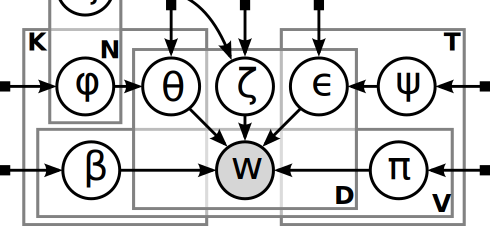
\includegraphics[width=0.5\linewidth]{fig/graphicalmodel.pdf}
% \caption{A directed graphical model of Capsule to show considered dependencies. Shaded document topics nodes $\theta$ are observed. unshaded nodes are hidden variables---these are event occurrences $\epsilon$, event content descriptions $\pi$, and entity typical concerns $\phi$. Plates denote replication: there are $D$ documents, $T$ time steps, $N$ entities, and $K$ topics. Hyperparameters $\eta$, $\mu$, and $\alpha$ are fixed.}
% \label{fig:graphicalmodel}
% \end{figure}

\begin{figure}
\begin{mdframed}
\small
\begin{itemize}[leftmargin=*]
\item for each time step $t=$~1:$T$,
	\begin{itemize}[leftmargin=*]
	\item draw event description over vocabulary \\$\pi_t \sim \mbox{Dirichlet}_V (\alpha)$
	\item draw event strength \\$\psi_{t} \sim \mbox{Gamma}(s_\psi, r_\psi)$
	\end{itemize}
\item for each topic $k=$~1:$K$,
	\begin{itemize}[leftmargin=*]
	\item draw topic distribution over vocabulary \\$\beta_k \sim \mbox{Dirichlet}_V (\alpha)$
	\item for each entity $n=$~1:$N$,
		\begin{itemize}[leftmargin=*]
		\item draw entity concern \\$\phi_{n,k} \sim \mbox{Gamma}(s_\phi, r_\phi)$
		\end{itemize}
	\end{itemize}
\item for each document $d=$~1:$D$ sent at time $i_d$ by author $a_d$,
	\begin{itemize}[leftmargin=*]
		\item for each topic $k=$~1:$K$,
		\begin{itemize}[leftmargin=*]
			\item draw local entity concern \\$\theta_{d,k} \sim \mbox{Gamma}(s_\theta, \phi_{a_d,k})$
		\end{itemize}
	\item for each time $t=$~1:$T$,
		\begin{itemize}[leftmargin=*]
			\item draw local event relevancy \\$\epsilon_{d,t} \sim \mbox{Gamma}(s_\epsilon, \psi_{i_d,t})$ 
		\end{itemize}
	\item for each vocabulary term $v=$~1:$V$,
		\begin{itemize}[leftmargin=*]
			\item draw word counts $w_{d,v} \sim\\ \mbox{Poisson}\left(\theta_d^\top\beta_v + \sum_{t=1}^T f(i_d, t) \epsilon_{d,t} \pi_{t,v}\right)$
		\end{itemize}
	\end{itemize}
\end{itemize}
\end{mdframed}
\caption{The generative process for Capsule.}
\label{fig:generative-model}
\end{figure}


\parhead{Learning the hidden variables.}
In order to use the Capsule model to explore the observed documents, we must compute the posterior distribution.  Conditional on the observed word counts $w$, our goals to to compute the posterior values of the hidden parameters---global event strengths $\psi$, event descriptions $\pi$, entity concerns $\phi$, and topics $\beta$, as well as document-specific entity concerns $\theta$ and event relevancy parameters $\epsilon$.

As for many Bayesian models, the exact posterior for Capsule is not tractable to compute; approximating it is our central statistical and computational problem.  We develop an approximate inference algorithm for Capsule based on variational methods~\cite{Wainwright:2008}.\footnote{Source code is available at https://github.com/?????/capsule.}

Variational inference approaches the problem of posterior inference by minimizing the KL divergence from an approximating distribution $q$ to the true posterior $p$.
This is equivalent to maximizing the ELBO,
\begin{multline}
	\mathcal{L}(q)  = \E_{q(\psi, \pi, \phi, \beta, \theta, \epsilon)}\bigl[\log p(w, \psi, \pi, \phi, \beta, \theta, \epsilon) \\
	-~\log q(\psi, \pi, \phi, \beta, \theta, \epsilon)\bigr].
	\label{eq:elbo}
\end{multline}

We define the approximating distribution $q$ using the mean field assumption:
\begin{multline}
	q(\psi, \pi, \phi, \beta, \theta, \epsilon) = \prod_{t=1}^T \left[ q(\pi_{t} \g \lambda^\pi_t) q(\psi_t \g \lambda^\psi_t) \right] \\
		\prod_{k=1}^K \left[ q(\beta_{k} \g \lambda^\beta_k) \prod_{n=1}^N q(\phi_{n,k} \g \lambda^\phi_{n,k}) \right] \\
		\prod_{d=1}^D \left[
				\prod_{k=1}^K q(\theta_{d,k} \g \lambda^\theta_{d,k})
				\prod_{t=1}^T q(\epsilon_{d,t} \g \lambda^\epsilon_{d,t})
			\right]
	\label{eq:q}
\end{multline}

The variational distributions $q(\pi)$ and $q(\beta)$ are both Dirichlet-distributed with free variational parameters $\lambda^\pi$ and $\lambda^\beta$, respectively.  Similarly, $q(\psi)$, $q(\phi)$, $q(\theta)$ and $q(\epsilon)$ are all gamma-distributed with corresponding free variational parameters $\lambda^\psi$, $\lambda^\phi$, $\lambda^\theta$, and $\lambda^\epsilon$.

The expectations under $q$, which are needed to maximize the ELBO, have closed form analytic updates, as detailed in Appendix~\ref{sec:inference}. We update each parameter in turn, following standard coordinate ascent variational inference techniques.  Full details on our inference algorithm can be found in the appendix.  This algorithm produces a fitted variational distribution which can then be used as a proxy for the true posterior, allowing us to explore a collection of documents with Capsule.  

\parhead{Visualization.}
Capsule is a high-level statistical tool. In order to understand and explore its results, a user must scrutinize numerical distributions.
To make Capsule more accessible, we developed an open source tool for visualizing its results.\footnote{Source code: https://github.com/?????/capsule-viz.}  Our tool creates a navigator of the documents and latent parameters, allowing users to explore events, entities, topics, and the original documents.  Figure~\ref{fig:viz} shows several screenshots of this browsing interface.

\begin{figure}
\centering
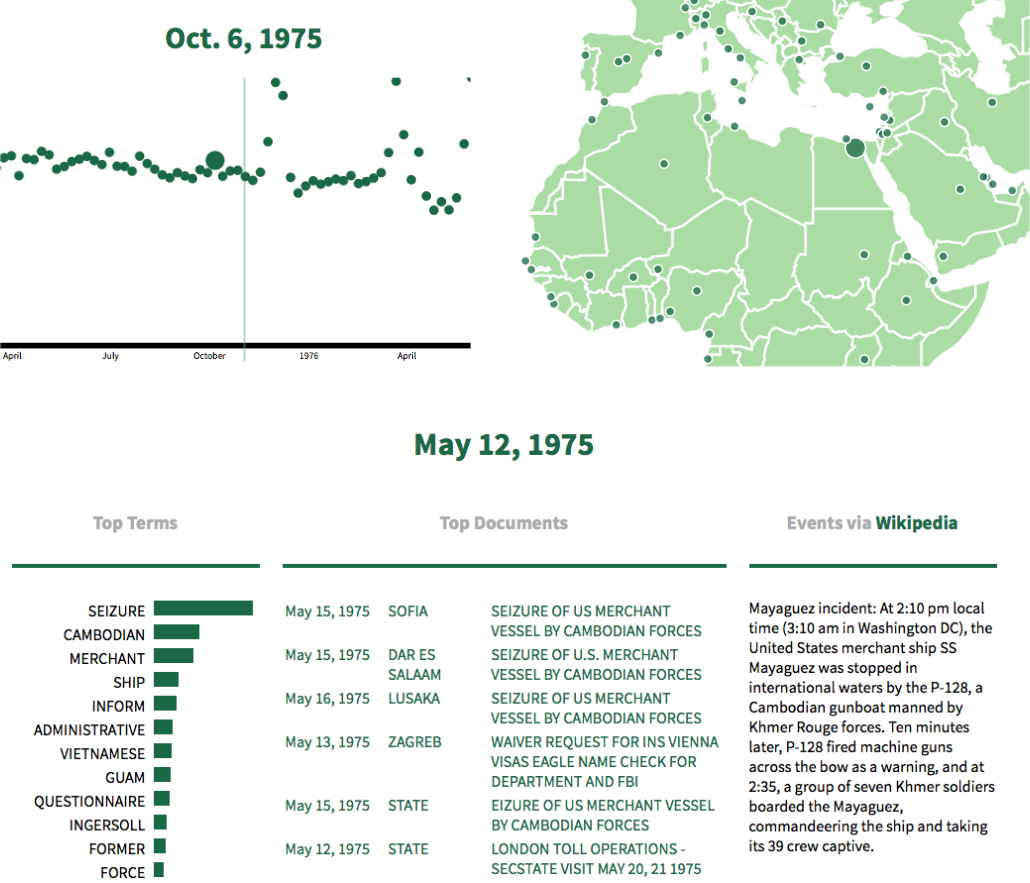
\includegraphics[width=\linewidth]{fig/viz.png}
\caption{Screenshots of Capsule visualization of US State Department cables.  Left: top words in a topic (manually labeled topic title).  Center-top: events over time (height is volume of messages sent, color is probability of an event occurring).  Center-bottom: topics for an event on <date TODO: cyprus coup?>.  Right-top: cyprus entity topics? TODO.  Right-bottom: entities shown on a map.}
\label{fig:viz}
\end{figure}


\section{Evaluation}
\label{sec:eval}
\PP outline two datasets (cables and enron) and the tasks to be done

\subsection{Data}
\parhead{Cables}

\parhead{arXiv}

\parhead{Enron}


\PP insert table and refetence for both (number of days, entities, total messages, or something); maybe a plot showing attributes of the data...somehow inform them that the state department is a bias for the cables data

\PP footnote on handling multiple recipients of message...

\subsection{Metrics and competing methods}

\PP how we evaluate based on real events

\PP how we evaluate based on perplexity (prediction of words)

\PP competing methods for perplexity: LDA, average user words?, dynamic topic model, network topic models

\subsection{Performance and exploration}

\PP sumry of comparison to gold-standard events for cables

\PP table of predictive likelihood results and summary pgh; and/or cite tea leaves paper

\parhead{Exploration}

\PP charachetrize events manually (based on cables) vs event detection characterization

\PP show descriptions for cables entities and select events; same for arxiv/enron

\PP any other exploration you can think of!


Results: ROC curve (x=false postive rate, y=true postive rate)


% push experimental details into a section at the end if needed

\section{Discussion}
\label{sec:discussion}
%!TEX root = emnlp2016.tex

We presented Capsule, a Bayesian model for detecting and
characterizing potentially significant events. We evaluated Capsule's
ability to detect events and find relevant messages; it outperformed four 
baseline methods. We used Capsule to analyze a large corpus of U.S. State 
Department cables from the 1970s, demonstrating 
that it can discover both well-known and obscure (but 
significant) events, as well as relevant documents;
this is increasingly important---it
is estimated that the State Department 
produces two billion e-mails annually. 
We anticipate that Capsule, and our
visualization tool, will be useful for historians, political
scientists, and journalists who wish to explore and understand large
corpora of documents.



% \subsection{Citations}
% Citations to articles \cite{bowman:reasoning,
% clark:pct, braams:babel, herlihy:methodology},
% conference proceedings \cite{clark:pct} or
% books \cite{salas:calculus, Lamport:LaTeX} listed
% in the Bibliography section of your
% article will occur throughout the text of your article.
% You should use BibTeX to automatically produce this bibliography;
% you simply need to insert one of several citation commands with
% a key of the item cited in the proper location in
% the \texttt{.tex} file \cite{Lamport:LaTeX}.
% The key is a short reference you invent to uniquely
% identify each work; in this sample document, the key is
% the first author's surname and a
% word from the title.  This identifying key is included
% with each item in the \texttt{.bib} file for your article.

% The details of the construction of the \texttt{.bib} file
% are beyond the scope of this sample document, but more
% information can be found in the \textit{Author's Guide},
% and exhaustive details in the \textit{\LaTeX\ User's
% Guide}\cite{Lamport:LaTeX}.

% This article shows only the plainest form
% of the citation command, using \texttt{{\char'134}cite}.
% This is what is stipulated in the SIGS style specifications.
% No other citation format is endorsed or supported.

% \subsection{Tables}
% Because tables cannot be split across pages, the best
% placement for them is typically the top of the page
% nearest their initial cite.  To
% ensure this proper ``floating'' placement of tables, use the
% environment \textbf{table} to enclose the table's contents and
% the table caption.  The contents of the table itself must go
% in the \textbf{tabular} environment, to
% be aligned properly in rows and columns, with the desired
% horizontal and vertical rules.  Again, detailed instructions
% on \textbf{tabular} material
% is found in the \textit{\LaTeX\ User's Guide}.

% Immediately following this sentence is the point at which
% Table 1 is included in the input file; compare the
% placement of the table here with the table in the printed
% dvi output of this document.

% \begin{table}
% \centering
% \caption{Frequency of Special Characters}
% \begin{tabular}{|c|c|l|} \hline
% Non-English or Math&Frequency&Comments\\ \hline
% \O & 1 in 1,000& For Swedish names\\ \hline
% $\pi$ & 1 in 5& Common in math\\ \hline
% \$ & 4 in 5 & Used in business\\ \hline
% $\Psi^2_1$ & 1 in 40,000& Unexplained usage\\
% \hline\end{tabular}
% \end{table}

% \begin{table*}
% \centering
% \caption{Some Typical Commands}
% \begin{tabular}{|c|c|l|} \hline
% Command&A Number&Comments\\ \hline
% \texttt{{\char'134}alignauthor} & 100& Author alignment\\ \hline
% \texttt{{\char'134}numberofauthors}& 200& Author enumeration\\ \hline
% \texttt{{\char'134}table}& 300 & For tables\\ \hline
% \texttt{{\char'134}table*}& 400& For wider tables\\ \hline\end{tabular}
% \end{table*}


% \begin{figure}
% \centering
% \includegraphics[height=1in, width=1in]{rosette}
% \caption{A sample black and white graphic that has
% been resized with the \texttt{includegraphics} command.}
% \vskip -6pt
% \end{figure}


% NOTE page limit: 10 pages max, including figures, references, and appendices

%ACKNOWLEDGMENTS are optional
%$\section{Acknowledgments}
%TODO
%
% The following two commands are all you need in the
% initial runs of your .tex file to
% produce the bibliography for the citations in your paper.
\bibliographystyle{abbrv}
\bibliography{library.bib} % sigproc.bib is the name of the Bibliography in this case
% You must have a proper ".bib" file
%  and remember to run:
% latex bibtex latex latex
% to resolve all references
%
% ACM needs 'a single self-contained file'!
%
%\balancecolumns
\appendix
In this appendix, we describe the details of the variational inference algorithm for Capsule. This algorithm fits the parameters of the variational distribution $q$ in Eq.~\ref{eq:q} so that it is close in KL divergence to the posterior.

Recall that the variational distributions $q(\pi)$ and $q(\phi)$ are both gamma-distributed with free variational parameters $\lambda^\pi$ and $\lambda^\phi$, respectively.  Each parameter $\lambda$ has two components: sparsity $\alpha$ and mean $\mu$, which parameterize a shape-rate gamma as $\mbox{Gamma}(\alpha,\mu/\alpha)$, as noted previously. Because these parameters are free, we use the softplus function $\mathcal{P}(x) = \log(1+\exp(x))$ to constrain them so that they do not violate the requirements of the gamma distribution.
The variational distribution $q(\epsilon)$ is Poisson-distributed with variational parameter $\lambda^\epsilon$, which is also constrained by the softplus function.

Minimizing the KL divergence between the true posterior $p$ and the variational approximation $q$ is equivalent to maximizing the ELBO (Eq.~\ref{eq:elbo}).  This maximization is often achieved with closed form coordinate updates, but the Capsule model is not specified with the required conjugate relationships that make this approach possible~\cite{Ghahramani:2001}.  Instead, we rely on ``black box'' variational inference techniques~\cite{Ranganath:2014} to perform this optimization.

Black box techniques optimize the ELBO directly with stochastic optimization, which maximizes a function using noisy estimates of its gradient~\cite{Robbins:1951}.  In this case, the function is the ELBO, and we take derivatives with respect to each of the variational parameters.  To obtain the noisy estimates, we sample from the variational approximation $q$; these samples then give us the noisy, unbiased gradients used to update our parameters.

It is essential to employ variance reducing techniques; without them, the algorithm would converge too slowly to be of practical value.  Details on each of these techniques may be found in the original black box variational inference paper~\cite{Ranganath:2014}.

One of these techniques is Rao-Blackwellization~\cite{Casella:1996}: for each variable, we can write the log probability of all terms containing that variable, giving us 
\[\log p^\epsilon_{t} \triangleq \log p(\epsilon_{t} \g \eta_\epsilon) + \sum_{d\in D_t}\sum_k\log p(\theta_{d,k} \g \cdots),\footnotemark\]
\footnotetext{Note that we abbreviate \[p^\epsilon_t = p^\epsilon_{t}(\theta, \epsilon, \pi, \phi)\] and 
\[p(\theta_{d,k} \g \cdots) = p(\theta_{d,k} \g \epsilon_t, \pi_{t,k}, \phi_{n_d,k}, \alpha_\theta),\]
and define
\[D_t \triangleq \forall d \in D : f(t, m_d) \neq 0.\]
}
\[\log p^\pi_{t,k} \triangleq \log p(\pi_{t,k} \g \mu_\pi, \alpha_\pi) + \mathbf{1}_{\epsilon_t} \sum_{d\in D_t}\log p(\theta_{d,k} \g \cdots),\footnotemark\]
\footnotetext{We use the indicator shorthand: 
\[\mathbf{1}_{\epsilon_t}=
\begin{cases}
  0, & \mbox{if } \epsilon_t = 0 \\
  1, & \mbox{otherwise.}
\end{cases}\]}
and
\[\log p^\phi_{n,k} \triangleq \log p(\phi_{n,k} \g \mu_\phi, \alpha_\phi) + \sum_{d\in D} \log p(\theta_{d,k} \g \cdots).\]
Then we can write the gradients with respect to the variational parameters as:
\[\nabla_{\lambda^\epsilon_{t}} \mathcal{L} = \E_q \left[ \nabla_{\lambda^\epsilon_{t}} \log q^\epsilon_{t} \left( \log p^\epsilon_{t} - \log q^\epsilon_{t} \right)\right],\footnotemark\]
\footnotetext{We employ yet another abbreviation:\[q^\epsilon_{t} = q(\epsilon_{t} \g \lambda^\epsilon_{t}).\]}
\[\nabla_{\lambda^\pi_{t,k}} \mathcal{L} = \E_q \left[ \nabla_{\lambda^\pi_{t,k}} \log q^\pi_{t,k} \left( \log p^\pi_{t,k} - \log q^\pi_{t,k} \right)\right],\]
and
\[\nabla_{\lambda^\phi_{n,k}} \mathcal{L} = \E_q \left[ \nabla_{\lambda^\phi_{n,k}} \log q^\phi_{n,k} \left( \log p^\phi_{n,k} - \log q^\phi_{n,k} \right)\right].\]

Using these gradients, we construct our black box algorithm below in Algorithm 1.  As shown, the algorithm does not subsample documents, but for large corpora, we subsample $B$ documents at each iteration and scale the contribution of these samples by $D/B$.

While not shown explicitly in Algorithm 1, we also use control variates and RMSProp~\cite{Dauphin:2015} to reduce variance.\footnote{In a conversation with Ranganath, he suggested replacing AdaGrad with RMSprop in setting the learning rate.}
Additionally, we truncate in two instances: sampled gamma variables are given a lower bound to avoid sampling too close to zero, and free parameters are given both lower and upper bounds---the latter is to avoid overflow.

\parhead{For Reference}
The gamma distribution and derivatives:
\begin{align}
\log\mbox{Gamma}(x \g \mu, \alpha) = & 
\alpha\log\alpha - \alpha\log\mu - \log\Gamma \left(\alpha\right)\nonumber \\
& + (\alpha-1)\log x - \frac{\alpha x}{\mu}, \label{eq:gamma} \\
\nabla_\mu \log\mbox{Gamma}(x \g \mu, \alpha) =&
-\frac{\alpha}{\mu} + \frac{\alpha x}{\mu^2},\label{eq:dgammaMu} \\
\nabla_\alpha \log\mbox{Gamma}(x \g \mu, \alpha) =& 
\log\alpha + 1 - \log\mu - \Psi \left(\alpha\right) \nonumber \\
& + \log x - \frac{x}{\mu}. \label{eq:dgammaAlpha}%was dgammaA
\end{align}

The Poisson distribution and derivative:
\begin{align}
\log\mbox{Poisson}(x~\vert~\lambda) &= x\log\lambda - \log(x!) - \lambda, \label{eq:poisson} \\
%\log\mbox{Poisson}(x~\vert~\mathcal{P}(\lambda)) &= x\log\mathcal{P}(\lambda) - \log(x!) -\mathcal{P}(\lambda) \\
\nabla_\lambda \log\mbox{Poisson}(x~\vert~\lambda) &= \frac{x}{\lambda} -1.\label{eq:dpoisson}
\end{align}

The softplus function and derivative:
\[\mathcal{P}(x) = \log(1+e^x),\]
\begin{equation}
\mathcal{P}'(x) = \frac{e^x}{1+e^x}.
\label{eq:dsoftplus}
\end{equation}

Note that the derivatives in Equations~\ref{eq:dgammaMu},~\ref{eq:dgammaAlpha}, and~\ref{eq:dpoisson} will always be used in conjunction with Equation~\ref{eq:dsoftplus}, as part of the chain rule:
\begin{equation}
\frac{d}{dx} f(\mathcal{P}(x)) = \mathcal{P}'(x)f'(\mathcal{P}(x)).
\label{eq:chain}
\end{equation}



\begin{algorithm}
\small
\DontPrintSemicolon
\KwIn{document topics $\theta$}
\KwOut{estimates of latent parameters event occurrences $\epsilon$, event topics $\pi$, and entity topics $\phi$}
\textbf{Initialize} $\lambda^\epsilon$, $\lambda^\phi$, and $\lambda^\pi$ to respective priors \;
\textbf{Initialize} iteration count $i = 0$ and $\sigma^\pi = 0$ \;
\While {change in validation likelihood $< \Delta$}{
  \For {each sample $s = 1, \dots, S$}{
    \For {each entity $n$ and component $k$} {
      draw sample entity topics $\phi_{n,k}[s] \sim \mbox{Gamma}(\mathcal{P}(\lambda^\phi_{n,k}))$ \;
      \BlankLine
      set $p$, $q$, and $g$ using Equations~\ref{eq:gamma}--\ref{eq:dgammaAlpha},~\ref{eq:dsoftplus}, and~\ref{eq:chain}: \;
      $p^\phi_{n,k}[s] = \log p(\phi_{n,k}[s] \g \mu_\phi, \alpha_\phi)$ \;
      $q^\phi_{n,k}[s] = \log q(\phi_{n,k}[s] \g \mathcal{P}(\lambda^\phi_{n,k}))$ \;
      $g^\phi_{n,k}[s] = \nabla_{\lambda^\phi_{n,k}} \log q(\phi_{n,k}[s] \g \mathcal{P}(\lambda^\phi_{n,k}))$ \;
    }
    \For {each time step $t$} {
      draw sample event occurrence $\epsilon_t[s] \sim \mbox{Poisson}(\mathcal{P}(\lambda^\epsilon_t))$ \;
      \BlankLine
      set $p$, $q$, and $g$ using Equations~\ref{eq:poisson}--\ref{eq:chain}: \;
      $p^\epsilon_i[s] = \log p(\epsilon_{i}[s] \g \eta)$ \;
      $q^\epsilon_i[s] = \log q(\epsilon_i[s] \g \mathcal{P}(\lambda^\epsilon_i))$ \;
      $g^\pi_{i}[s] = \nabla_{\lambda^\epsilon_{i}} \log q(\epsilon_{i}[s] \g \mathcal{P}(\lambda^\epsilon_{i}))$ \;
      \BlankLine
      \If {$\epsilon_i[s] \neq 0$} {
        \For {each component $k$} {
          draw sample event topics $\pi_{t,k}[s] \sim \mbox{Gamma}(\mathcal{P}(\lambda^\pi_{t,k}))$ \;
          \BlankLine
          set $p$, $q$, and $g$ using Equations~\ref{eq:gamma}--\ref{eq:dgammaAlpha},~\ref{eq:dsoftplus}, and~\ref{eq:chain}: \;
          $p^\pi_{ik}[s] = \log p(\pi_{ik}[s] \g \alpha_0, \beta_0)$ \;
          $q^\pi_{ik}[s] = \log q(\pi_{ik}[s] \g \lambda^\pi_{ik})$ \;
          $g^\pi_{ik}[s] = \nabla_{\lambda^\pi_{ik}} \log q(\pi_{ik}[s] \g \lambda^\pi_{ik})$ \;
        }
      }
    }
  }
  
  \For {each document $d$, sample $s$ and component $k$}{
    set $\mu_{d,k}[s] = \phi_{n_d,k}[s] + \sum_t f(t, m_d) \epsilon_t[s] \pi_{t,k}[s]$ \;
    set $p^\theta_{d,k}[s] = \log p(\theta_{d,k} \g \mu_{d,k}[s], \alpha_\theta)$ (Eqn.~\ref{eq:gamma})
    \BlankLine
    $p^\phi_{n,k}[s] \pluseq p^\theta_{n,k}[s]$ \;
    \For {each timestep $t$ where $t \le m_d < t + \delta$}{
      $p^\epsilon_{t}[s] \pluseq \sum_k p^\theta_{d,k}[s]$ \;
      \If {$\epsilon_t[s] \neq 0$} {
        $p^\pi_{t,k}[s] \pluseq p^\theta_{t,k}[s]$ \;
        update $\sigma^\pi_t \pluseq 1$ \;
      }
    }
  }

  
  set $\hat\nabla_{\lambda^{\phi} }\mathcal{L} \triangleq \frac{1}{S} \sum_s g^\phi[s] ( p^\phi[s] -  q^\phi[s] )$ \;
  set $\hat\nabla_{\lambda^{\epsilon}} \mathcal{L} \triangleq \frac{1}{S} \sum_s g^\epsilon[s] ( p^\epsilon[s] -  q^\epsilon[s] )$ \;
  set $\hat\nabla_{\lambda^{\pi}} \mathcal{L} \triangleq \frac{1}{\sigma_\pi} \sum_s g^\pi[s] ( p^\pi[s] -  q^\pi[s] )$ \;

  \BlankLine
  set $\rho= (t +\tau)^\kappa$ \;
  % update event content for each event $i$ and topic $k$: 
  set $\lambda^{\pi} \pluseq \rho \hat\nabla_{\lambda^{\pi}} \mathcal{L}$ \;
  set $\lambda^{\epsilon} \pluseq \rho \hat\nabla_{\lambda^{\epsilon}} \mathcal{L}$ \;
  set $\lambda^{\phi} \pluseq \rho \hat\nabla_{\lambda^{\phi}} \mathcal{L}$ \;
}

set $\E[\pi] = \lambda^{\pi,a}$ \;
set $\E[\phi] = \lambda^{\phi,a}$ \;
set $\E[\epsilon] = \lambda^{\epsilon}$ \;
\BlankLine
\Return{$\E[\pi]$, $\E[\phi]$, $\E[\epsilon]$} \;
\caption{Inference for Cables Model}
\label{alg:cables}
\end{algorithm}


\end{document}
